\documentclass{beamer}
\usepackage{tcolorbox}
\usepackage{forloop}
\usepackage{bm}

\usepackage{mathtools}
\mathtoolsset{showonlyrefs}  

%\beamerdefaultoverlayspecification{<+->}
\newcommand{\data}{\mathcal{D}}

\DeclareMathOperator*{\argmin}{arg\,min}

\newcommand\Item[1][]{%
	\ifx\relax#1\relax  \item \else \item[#1] \fi
	\abovedisplayskip=0pt\abovedisplayshortskip=0pt~\vspace*{-\baselineskip}}

\usetheme{metropolis}           % Use metropolis theme


\title{Multivariate Normal Distribution}
\date{\today}
\author{Nipun Batra}
\institute{IIT Gandhinagar}
\begin{document}
  \maketitle
  
  


\begin{frame}{Univariate Normal Distribution}

The probability density of univariate Gaussian is given as: $$f(x) = \frac{1}{\sigma \sqrt{2\pi} } e^{-\frac{1}{2}\left(\frac{x-\mu}{\sigma}\right)^2}$$
	
also, given as 
$$f(x)\sim \mathcal{N}(\mu, \sigma^2)$$

with mean $\mu \in R$ and variance $\sigma^2 >0$ 

\end{frame}

\begin{frame}{Univariate Normal Distribution}
Pop Quiz: Why is the denominator the way it is? Let the normalizing constant be $c$ and let $g(x) = e^{-\frac{1}{2}\left(\frac{x-\mu}{\sigma}\right)^2}$.

\begin{gather}
\visible<1->{1 = \int_{-\infty}^{\infty} c \cdot g(x) dx\\}
\visible<2->{1 = \int_{-\infty}^{\infty} ce^{-\frac{(x - u)^2}{2\sigma^2}} dx}
\end{gather}
\visible<3->{Let's substitute $\frac{x - u}{\sqrt{2}\sigma}$ with $t$.}
\begin{gather}
\visible<4->{1 = \int_{-\infty}^{\infty} ce^{-t^2} dt \times \sqrt{2}\sigma\\}
\visible<5->{1 = \sqrt{2}\sigma c \times 2\int_{0}^{\infty} e^{-t^2} dt}
\end{gather}
\end{frame}

\begin{frame}{Univariate Normal Distribution}
	$$ \frac{2}{\sqrt{\pi}}\int_{0}^{\infty} e^{-t^2} dt $$
	The above expression is called error function and is it's value is denoted by $erf(t)$. In our case, we want $erf(\infty)$ which is equal to 1.
	
	\begin{gather}
	\visible<2->{1 = \sqrt{2\pi}\sigma c \times \frac{2}{\sqrt{\pi}}\int_{0}^{\infty} e^{-t^2} dt\\}
	\visible<3->{1 = \sqrt{2\pi}\sigma c \times 1\\}
	\visible<4->{\frac{1}{\sqrt{2\pi}\sigma} = c}
	\end{gather}
\end{frame}

\begin{frame}{Univariate Normal Distribution}
	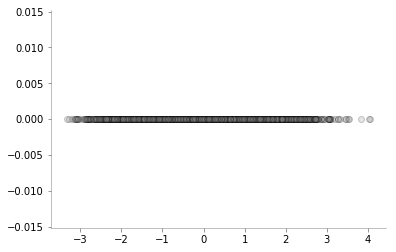
\includegraphics[width=\linewidth,height=\textheight,keepaspectratio]{gp/1d-gp} 
\end{frame}

\begin{frame}{Univariate Normal Distribution}
	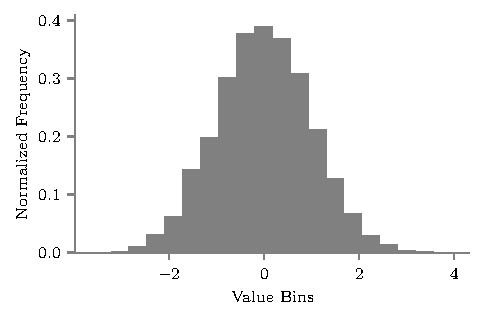
\includegraphics[width=\linewidth,height=\textheight,keepaspectratio]{gp/1d-gp-hist}
\end{frame}

%\begin{frame}{Univariate Normal Distribution}
%Add plots for 1d histogram with different bin-width
%\end{frame}

\begin{frame}{Univariate Normal Distribution}
	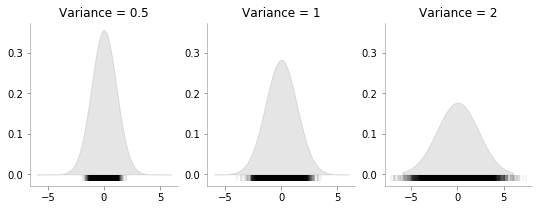
\includegraphics[width=\linewidth,height=\textheight,keepaspectratio]{gp/1d-gp-kde2}
\end{frame}


\begin{frame}{Bivariate Normal Distribution}
Bivariate normal distribution of two-dimensional random vector $\bf{X} =\begin{bmatrix}
X_{1} \\
X_{2} \\
\end{bmatrix}
$

\begin{gather}
	\bf{X} = \begin{pmatrix}
	X_1 \\
	X_2
	\end{pmatrix} \sim \mathcal{N}_2 (\mu , \Sigma)
\end{gather}

where, mean vector $\bm{\mu} =\begin{bmatrix}
\mu_{1} \\
\mu_{2} \\
\end{bmatrix}
=\begin{bmatrix}
\operatorname{E}[X_{1}] \\
\operatorname{E}[X_{2}] \\
\end{bmatrix}
$

and, covariance matrix $\Sigma$
$$\Sigma_{i,j} := \operatorname{E} [(X_i - \mu_i)( X_j - \mu_j)] = \operatorname{Cov}[X_i, X_j] $$
\end{frame}

\begin{frame}{Bivariate Normal Distribution}

Question: What is Cov(X, X)?

Answer: Var(X) = Cov(X, X) =  $\operatorname{E}[(X - \operatorname{E}[X])]^2$

In the case of univariate normal, Var(X) is written as $\sigma^2$

Question: What is the relation between $\Sigma_{i, j}$ and $\Sigma_{j, i}$?

Answer: They are the same!

Question: What can we say about the covariance matrix $\Sigma$?

Answer: It is symmetric. Thus $\Sigma = \Sigma^T$
\end{frame}

\begin{frame}{Correlation and Covariance}
If $X$ and $Y$ are two random variables, with means (expected values) $\mu_X$ and $\mu_Y$ and standard deviations $\sigma_X$ and $\sigma_Y$, respectively, then their covariance and correlation are as follows:

$$\text{cov}_{XY} = \sigma_{XY} = E[(X-\mu_X)\,(Y-\mu_Y)] $$

$$	\text{corr}_{XY} = \rho_{XY} = E[(X-\mu_X)\,(Y-\mu_Y)]/(\sigma_X \sigma_Y)
$$
so that
$$
\rho_{XY} = \sigma_{XY} / (\sigma_X \sigma_Y) $$

where $E$ is the expected value operator. 
\end{frame}

\begin{frame}{PDF of bivariate normal distribution}

We might have seen that 

$$f_X(X_1, X_2) = \frac{exp(\frac{-1}{2}(X-\mu)^T \Sigma^{-1}(X-\mu))}{2\pi |\Sigma|^\frac{1}{2}}$$

How do we get such a weird looking formula?!

\end{frame}

\begin{frame}{PDF of bivariate normal with no cross-correlation}

Let us assume no correlation between $X_1$ and $X_2$.

We have $\Sigma = \begin{bmatrix}
\sigma_1^2 & 0 \\
0 & \sigma_2^2 \\
\end{bmatrix}$

We have $f_X(X_1, X_2) = f_X(X_1)f_X(X_2)$

$$=\frac{1}{\sigma_1 \sqrt{2\pi} } e^{-\frac{1}{2}\left(\frac{X_1-\mu_1}{\sigma_1}\right)^2} \times \frac{1}{\sigma_2 \sqrt{2\pi} } e^{-\frac{1}{2}\left(\frac{X_2-\mu_2}{\sigma_2}\right)^2}$$

$$= \frac{1}{\sigma_1 \sigma_2 2\pi } e^{-\frac{1}{2}\{\left(\frac{X_1-\mu_1}{\sigma_1}\right)^2 + \left(\frac{X_2-\mu_2}{\sigma_2}\right)^2 \}}  $$
\end{frame}

\begin{frame}{PDF of bivariate normal with no cross-correlation}

Let us consider only the exponential part for now

$ Q =  \left(\frac{X_1-\mu_1}{\sigma_1}\right)^2 + \left(\frac{X_2-\mu_2}{\sigma_2}\right)^2 $

Question: Can you write Q in the form of vectors X and $\mu$?

$$
 = \begin{bmatrix}
	X_1 - \mu_1 &
	X_2 - \mu_2 \\
\end{bmatrix}_{1\times2}  g(\Sigma)_{2\times2} \begin{bmatrix}
X_1 - \mu_1 \\
X_2 - \mu_2 \\
\end{bmatrix}_{2\times1}
$$

Here $g(\Sigma)$ is a matrix function of $\Sigma$ that will result in $\sigma_1^2$ like terms in the denominator; also there is no cross-terms indicating zeros in right diagonal!

$g(\Sigma) = \begin{bmatrix}
 \frac{1}{\sigma_1^2}& 0  \\
 0 &  \frac{1}{\sigma_2^2} \\
\end{bmatrix}_{2\times2} = \frac{1}{\sigma_1^2 \sigma_2^2}\begin{bmatrix}
{\sigma_2^2}& 0  \\
0 &  {\sigma_1^2}   \\ 
\end{bmatrix}_{2\times2} = \frac{1}{|\Sigma|} \operatorname{adj(\Sigma)} = \Sigma^{-1}$
\end{frame}


\begin{frame}{PDF of bivariate normal with no cross-correlation}
Let us consider the normalizing constant part now.
$M = \frac{1}{\sigma_1 \sigma_2 2\pi }$
$=\frac{1}{2\pi \times |\Sigma|^{\frac{1}{2}}}$
\end{frame}


\begin{frame}{Bivariate Gaussian samples with cross-correlation  = 0}
	\begin{center}
		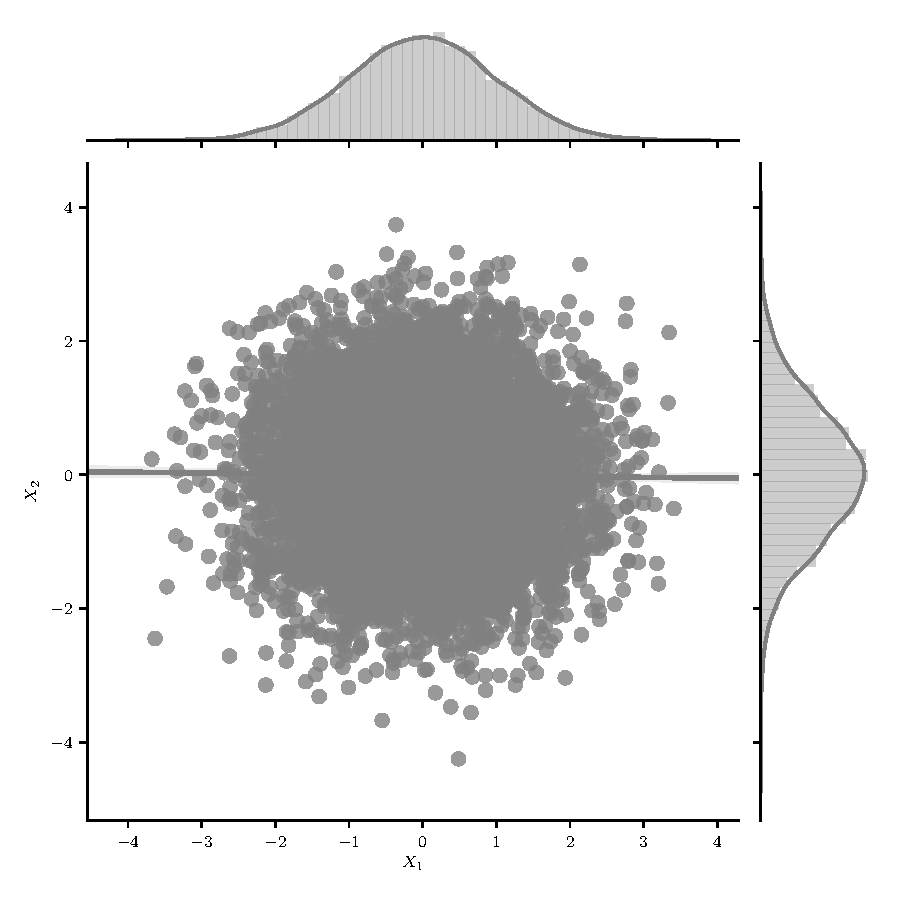
\includegraphics[width=\linewidth,height=\textheight - 10pt,keepaspectratio]{gp/2d-gp3}
	\end{center}
\end{frame}

\begin{frame}{Bivariate Gaussian samples with cross-correlation  $\neq$ 0}
	\begin{center}
		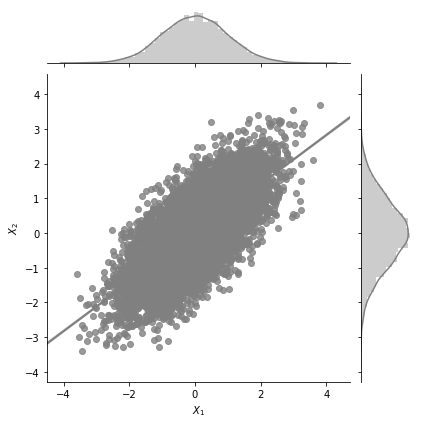
\includegraphics[width=\linewidth,height=\textheight - 10pt,keepaspectratio]{gp/2d-gp}
	\end{center}
\end{frame}


\urldef\nodeSix\url{http://fourier.eng.hmc.edu/e161/lectures/gaussianprocess/node6.html}
\urldef\nodeSeven\url{http://fourier.eng.hmc.edu/e161/lectures/gaussianprocess/node7.html}


\begin{frame}{Detour: Inverse of partioned symmetric matrix \footnote{Courtesy: \nodeSix}}

Consider an $n\times n$ symmetric matrix $A$ and divide it into four blocks

$
A = \begin{bmatrix}
	A_{11} & A_{12}\\
	A_{21} & A_{22} \\
\end{bmatrix} =  \begin{bmatrix}
A_{11} & A_{12}\\
A_{12}^T & A_{22} \\
\end{bmatrix}
$

For example, let $n=3$, we have

$$
A =  \begin{bmatrix}
	1 & 2 & 3\\
	2 & 5 & 6 \\
	3 & 6 & 8 \\
	
\end{bmatrix}
$$

We could for example have 

$A_{11} = \begin{bmatrix}
1 & 2 \\
2 & 5 \\
\end{bmatrix}$ and $A_{12} = \begin{bmatrix}
3 \\ 6
\end{bmatrix}
$ and $A_{22} = \begin{bmatrix}
8
\end{bmatrix}$
\end{frame}

\begin{frame}{Detour: Inverse of partioned symmetric matrix}
Question: Write $B = A^{-1}$ in terms of the four blocks
$
B = \begin{bmatrix}
	B_{11} & B_{12}\\
	B_{12}^T & A_{22} \\
\end{bmatrix}
= A^{-1}$

$A_{11}$ and $B_{11} \in R^{p\times p}$ 

$A_{22}$ and $B_{22} \in R^{q\times q}$

$A_{12} = A_{21}^T$ and $B_{12} = B_{21}^T \in R^{p\times q}$

and, p + q = n 
 
\end{frame}

\begin{frame}{Detour: Inverse of partioned symmetric matrix}
$I_n = AA^{-1} = AB$

$=\begin{bmatrix}
A_{11} & A_{12}\\
A_{12}^T & A_{22} \\
\end{bmatrix} \begin{bmatrix}
B_{11} & B_{12}\\
B_{12}^T & B_{22} \\
\end{bmatrix}
= \begin{bmatrix}
A_{11}B_{11} +A_{12}B_{12}^T & A_{11}B_{12} + A_{12}A_{22}\\
A_{12}^TB_{11} + A_{22}B_{12}^T & A_{12}^TB_{12} + A_{22}B_{22}  \\
\end{bmatrix} = \begin{bmatrix}
I_p & 0 \\
0 & I_q
\end{bmatrix}$

Thus, we have
\begin{gather}
A_{11}B_{11} +A_{12}B_{12}^T = I_p\\
A_{11}B_{12} + A_{12}A_{22} = 0^{p\times q}\\
A_{12}^TB_{11} + A_{22}B_{12}^T = 0^{q\times p}\\
A_{12}^TB_{12} + A_{22}B_{22} = I_q
\end{gather}
\end{frame}

\begin{frame}{Detour: Inverse of partioned symmetric matrix}
Moving the expressions around we get the following results.

\begin{gather}
	B_{11} = (A_{11} - A_{12}A_{22}^{-1}A_{12}^T)^{-1} = A_{11}^{-1} + A_{11}^{-1}A_{12}(A_{22} - A_{12}^TA_{11}^{-1}A_{12})^{-1}A_{12}^TA_{11}^{-1}\\
	B_{22} = (A_{22} - A_{12}^TA_{11}^{-1}A_{12})^{-1} = A_{22}^{-1} + A_{22}^{-1}A_{12}^T(A_{11} - A_{12}A_{22}^{-1}A_{12}^T)^{-1}A_{12}A_{22}^{-1}\\
	B_{12}^T = - A_{22}^{-1}A_{12}^T ( A_{11} - A_{12} A_{22}^{-1} A_{12}^T)^{-1}\\\\
	B_{12}^T = - A_{11}^{-1}A_{12}^T ( A_{22} - A_{12} ^TA_{11}^{-1} A_{12})^{-1}
\end{gather}
\end{frame}

\begin{frame}{Determinant of Partitioned Symmetric Matrix}
	
\textbf{Theorem:} Determinant of a partitioned symmetric matrix can be written as follows
	\begin{gather}
		\vert A \vert 
		= \bigg| 
		\begin{bmatrix}
			A_{11}&A_{12}\\
			A_{21}&A_{22}
		\end{bmatrix}
		\bigg| \\
		=\vert A_{11}\vert \vert A_{22}-A_{12}^TA_{11}^{-1}A_{12}\vert \\
		=\vert A_{22}\vert \vert
		 A_{11}-A_{12}A_{22}^{-1}A_{12}^T \vert 
	\end{gather}
\end{frame}

\begin{frame}{Determinant of Partitioned Symmetric Matrix}
\textbf{Proof:} Note that
	\begin{gather}
		A = 
		\begin{bmatrix}
			A_{11}&A_{12} \\
			A_{21}&A_{22}
		\end{bmatrix}
		= 
		\begin{bmatrix}
			A_{11}& 0 \\
			A_{12}^T& I
		\end{bmatrix}
		\begin{bmatrix}
			I & A_{11}^{-1}A_{12} \\
			0 & A_{22} - A_{12}^TA_{11}^{-1}A_{12}
		\end{bmatrix}\\
		= 
		\begin{bmatrix}
			I & A_{12} \\
			0 & A_{22}
		\end{bmatrix}
		\begin{bmatrix}
			A_{11} - A_{12}A_{22}^{-1}A_{12}^T & 0\\
			A_{22}^{-1}A_{21}  & I
		\end{bmatrix}
	\end{gather} 
	
The theorem is proved as we also know that
\begin{equation}
	\vert AB\vert=\vert A\vert  \vert B\vert 
\end{equation}

and
\begin{equation}
	\left\vert 
		\begin{matrix}
			B&0 \\
			C&D
		\end{matrix} 
	\right\vert
	=
	\left\vert 
		\begin{matrix}
			B&C \\
			0&D
		\end{matrix} 
	\right\vert
	=
	\vert B\vert\
	\vert D\vert 
\end{equation}	
\end{frame}

\begin{frame}{Marginalisation and Conditional of multivariate normal\footnote{Courtesy: \nodeSeven.}}
Assume an n-dimensional random vector

\begin{equation}
	{\bf x}=\begin{bmatrix}{\bf x}_1 & {\bf x}_2\end{bmatrix} 
\end{equation}

has a normal distribution $N({\bf x},\mu,\Sigma)$ with
\begin{gather}\mu=
	\begin{bmatrix}
		\mu_1 \\
		\mu_2
	\end{bmatrix} 
	\text{and }
	\Sigma = \begin{bmatrix}
		\Sigma_{11}& \Sigma_{12}\\
		\Sigma_{21}&\Sigma_{22}
	\end{bmatrix} 
\end{gather}

where ${\bf x}_1$ and ${\bf x}_2$ are two subvectors of respective dimensions $p$ and $q$ with $p+q=n$. Note that $\Sigma=\Sigma^T$, and $\Sigma_{21}=\Sigma_{21}^T$.
\end{frame}

\begin{frame}{Marginalisation and Conditional of multivariate normal}
\textbf{Theorem:}

\textbf{part a:} The marginal distributions of ${\bf x}_1$ and ${\bf x}_2$ are also normal with mean vector $\mu_i$ and covariance matrix $\Sigma_{ii}$ ($i=1,2$), respectively.

\textbf{part b:} The conditional distribution of ${\bf x}_i$ given ${\bf x}_j$ is also normal with mean vector

\end{frame}

\begin{frame}{Marginalisation and Conditional of multivariate normal}
	\textbf{Proof:}
	
	The joint density of ${\bf x}$ is:
	
	\begin{equation}
	f({\bf x})=f({\bf x}_1,{\bf x}_2)=\frac{1}{(2\pi)^{n/2\vert\Sigma\vert^{1/2}}}exp[-\frac{1}{2}Q({\bf x}_1,{\bf x}_2)] 
	\end{equation}
	
	where $Q$ is defined as
	\begin{gather}
		Q({\bf x}_1,{\bf x}_2) = ({\bf x}-\mu)^T\Sigma^{-1}({\bf x}-\mu)\\
		= [({\bf x}_1-\mu_1)^T, ({\bf x}_2-\mu_2)^T] 
		\begin{bmatrix}
			\Sigma^{11} & \Sigma^{12}\\
			\Sigma^{21} & \Sigma^{22}
		\end{bmatrix}
		\begin{bmatrix}
			{\bf x}_1-\mu_1 \\
			{\bf x}_2-\mu_2
		\end{bmatrix}\\
		= ({\bf x}_1-\mu_1)^T\Sigma^{11}({\bf x}_1-\mu_1)+ 2({\bf x}_1-\mu_1)^T\Sigma^{12}({\bf x}_2-\mu_2) + ({\bf x}_2-\mu_2)^T \cdots \\
		\cdots \Sigma^{22}({\bf x}_2-\mu_2)
	\end{gather}
\end{frame}

\begin{frame}{Marginalisation and Conditional of multivariate normal}
	Here we have assumed 
$$	
	\Sigma^{-1}=\left[\begin{array}{cc}
		{\Sigma_{11}} & {\Sigma_{12}} \\
		{\Sigma_{21}} & {\Sigma_{22}}
	\end{array}\right]^{-1}=\left[\begin{array}{cc}
		{\Sigma^{11}} & {\Sigma^{12}} \\
		{\Sigma^{21}} & {\Sigma^{22}}
	\end{array}\right]
$$

	According to inverse of a partitioned symmetric matrix we have, 
	\begin{gather}
		\Sigma^{11}=\left(\Sigma_{11}-\Sigma_{12} \Sigma_{22}^{-1} \Sigma_{12}^{T}\right)^{-1}=\Sigma_{11}^{-1}+\Sigma_{11}^{-1} \Sigma_{12}\left(\Sigma_{22}-A_{12}^{T} \Sigma_{11}^{T} \Sigma_{12}\right)^{-1} \Sigma_{12}^{T} \Sigma_{11}^{-1}\\
		\Sigma^{22}=\left(\Sigma_{22}-\Sigma_{12}^{T} \Sigma_{11}^{-1} \Sigma_{12}\right)^{-1}=\Sigma_{22}^{-1}+\Sigma_{22}^{-1} \Sigma_{12}^{T}\left(\Sigma_{11}-\Sigma_{12} \Sigma_{22}^{-1} \Sigma_{12}^{T}\right)^{-1} \Sigma_{12} \Sigma_{22}^{-1}\\
		\Sigma^{12}=-\Sigma_{11}^{-1} \Sigma_{12}\left(\Sigma_{22}-\Sigma_{12}^{T} \Sigma_{11}^{-1} \Sigma_{12}\right)^{-1}=\left(\Sigma^{21}\right)^{T}
	\end{gather}

\end{frame}

\begin{frame}{Marginalisation and Conditional of multivariate normal}
	Substituting the second expression for $\Sigma^{11}$, first expression for $\Sigma^{22}$, and $\Sigma^{12}$ into $Q({\bf x}_1,{\bf x}_2)$ to get:
	
	\begin{gather}
	\begin{aligned}
	Q\left(\mathbf{x}_{1}, \mathbf{x}_{2}\right)=&\left(\mathbf{x}_{1}-\mu_{1}\right)^{T}\left[\Sigma_{11}^{-1}+\Sigma_{11}^{-1} \Sigma_{12}\left(\Sigma_{22}-A_{12}^{T} \Sigma_{11}^{-1} \Sigma_{12}\right)^{-1} \Sigma_{12}^{T} \Sigma_{11}^{-1}\right]\left(\mathbf{x}_{1}-\mu_{1}\right) \\
	&-2\left(\mathbf{x}_{1}-\mu_{1}\right)^{T}\left[\Sigma_{11}^{-1} \Sigma_{12}\left(\Sigma_{22}-\Sigma_{12}^{T} \Sigma_{11}^{-1} \Sigma_{12}\right)^{-1}\right]\left(\mathbf{x}_{2}-\mu_{2}\right) \\
	&+\left(\mathbf{x}_{2}-\mu_{2}\right)^{T}\left[\left(\Sigma_{22}-\Sigma_{12}^{T} \Sigma_{11}^{-1} \Sigma_{12}\right)^{-1}\right]\left(\mathbf{x}_{2}-\mu_{2}\right)\\
	=&\left(\mathbf{x}_{1}-\mu_{1}\right)^{T} \Sigma_{11}^{-1}\left(\mathbf{x}_{1}-\mu_{1}\right) \\
	&\left.+\left(\mathbf{x}_{1}-\mu_{1}\right)^{T} \Sigma_{11}^{-1} \Sigma_{12}\left(\Sigma_{22}-A_{12}^{T} \Sigma_{11}^{-1} \Sigma_{12}\right)^{-1} \Sigma_{12}^{T} \Sigma_{11}^{-1}\right]\left(\mathbf{x}_{1}-\mu_{1}\right) \\
	&-2\left(\mathbf{x}_{1}-\mu_{1}\right)^{T}\left[\Sigma_{11}^{-1} \Sigma_{12}\left(\Sigma_{22}-\Sigma_{12}^{T} \Sigma_{11}^{-1} \Sigma_{12}\right)^{-1}\right]\left(\mathbf{x}_{2}-\mu_{2}\right) \\
	&+\left(\mathbf{x}_{2}-\mu_{2}\right)^{T}\left[\left(\Sigma_{22}-\Sigma_{12}^{T} \Sigma_{11}^{-1} \Sigma_{12}\right)^{-1}\right]\left(\mathbf{x}_{2}-\mu_{2}\right)
	\end{aligned}\\
	\end{gather})
\end{frame}

\begin{frame}{Marginalisation and Conditional of multivariate normal}
	\begin{gather}
	\begin{aligned}
	=&\left(\mathbf{x}_{1}-\mu_{1}\right)^{T} \Sigma_{11}^{-1}\\
	&+\left[\left(\mathbf{x}_{2}-\mu_{2}\right)-\Sigma_{12}^{T} \Sigma_{11}^{-1}\left(\mathbf{x}_{1}-\mu_{1}\right)\right]^{T}\left(\Sigma_{22}-\Sigma_{12}^{T} \Sigma_{11}^{-1} \Sigma_{12}\right)^{-1}\left[\left(\mathbf{x}_{2}-\mu_{2}\right)-\Sigma_{12}^{T} \Sigma_{11}^{-1}\left(\mathbf{x}_{1}-\mu_{1}\right)\right]
	\end{aligned}
	\end{gather}
	The last equal sign is due to the following equations for any vectors $u$ and $v$ and a symmetric matrix $A=A^T$:
	
	\begin{gather}
		\begin{aligned}
		& u^{T} A u-2 u^{T} A v+v^{T} A v=u^{T} A u-u^{T} A v-u^{T} A v+v^{T} A v \\
		=& u^{T} A(u-v)-(u-v)^{T} A v=u^{T} A(u-v)-v^{T} A(u-v) \\
		=&(u-v)^{T} A(u-v)=(v-u)^{T} A(v-u)
		\end{aligned} 
	\end{gather}
\end{frame}

\begin{frame}{Marginalisation and Conditional of multivariate normal}
	We define  
	$b \triangleq \mu_{2}+\Sigma_{12}^{T} \Sigma_{11}^{-1}\left(\mathbf{x}_{1}-\mu_{1}\right)$
	\[
	A \triangleq \Sigma_{22}-\Sigma_{12}^{T} \Sigma_{11}^{-1} \Sigma_{12}
	\]
	
	and 
	$$\left\{\begin{array}{l}{Q_{1}\left(\mathrm{x}_{1}\right) \quad \triangleq\left(\mathrm{x}_{1}-\mu_{1}\right)^{T} \Sigma_{1}^{-1}\left(\mathrm{x}_{1}-\mu_{1}\right)} \\ {Q_{2}\left(\mathrm{x}_{1}, \mathrm{x}_{2}\right) \triangleq\left[\left(\mathrm{x}_{2}-\mu_{2}\right)-\Sigma_{12}^{T} \Sigma_{11}^{-1}\left(\mathrm{x}_{1}-\mu_{1}\right)\right]^{T}\left(\Sigma_{22}-\Sigma_{12}^{T} \Sigma_{11}^{-1} \Sigma_{12}\right)^{-1}\left[\left(\mathrm{x}_{2}-\mu_{2}\right)-\Sigma_{12}^{T} \Sigma_{11}^{-1}\left(\mathrm{x}_{1}-\mu_{1}\right)\right]} \\ {=\left(\mathrm{x}_{2}-b\right)^{T} A^{-1}\left(\mathrm{x}_{2}-b\right)}\end{array}\right.$$
	
	and get 
	$$Q\left(\mathbf{x}_{1}, \mathbf{x}_{2}\right)=Q_{1}\left(\mathbf{x}_{1}\right)+Q_{2}\left(\mathbf{x}_{1}, \mathbf{x}_{2}\right)$$
\end{frame}


\begin{frame}{Marginalisation and Conditional of multivariate normal}
	Now the joint distribution can be written as: 
	
	$$\begin{aligned} f(\mathrm{x}) &=f\left(\mathrm{x}_{1}, \mathrm{x}_{2}\right)=\frac{1}{(2 \pi)^{n / 2}\vert\Sigma\vert^{1 / 2}} \exp \left[-\frac{1}{2} Q\left(\mathrm{x}_{1}, \mathrm{x}_{2}\right)\right] \\ &=\frac{1}{(2 \pi)^{n / 2}\left|\Sigma_{11}\right|^{1 / 2}\left|\Sigma_{22}-\Sigma_{12}^{T} \Sigma_{11}^{-1} \Sigma_{12}\right|^{1 / 2}} \exp \left[-\frac{1}{2} Q\left(\mathrm{x}_{1}, \mathrm{x}_{2}\right)\right] \\ &=\frac{1}{(2 \pi)^{p / 2}\left|\Sigma_{11}\right|^{1 / 2}} \exp \left[-\frac{1}{2}\left(\mathrm{x}_{1}-\mu_{1}\right)^{T} \Sigma_{11}^{-1}\left(\mathrm{x}_{1}-\mu_{1}\right)\right] \frac{1}{(2 \pi)^{q / 2}|A|^{1 / 2}} \exp \left[-\frac{1}{2}\left(\mathrm{x}_{2}-b\right)^{T} A^{-1}\left(\mathrm{x}_{2}-b\right)\right] \\ &=N\left(\mathrm{x}_{1}, \mu_{1}, \Sigma_{11}\right) N\left(\mathrm{x}_{2}, b, A\right) \end{aligned}$$
	
	The third equal sign is due to Determinant of a partitioned symmetric matrix:
	
	$|\Sigma|=\left|\Sigma_{11}\right|\left|\Sigma_{22}-\Sigma_{12}^{T} \Sigma_{11}^{-1} \Sigma_{12}\right|$
\end{frame}

\begin{frame}{Marginalisation and Conditional of multivariate normal}
	The marginal distribution of ${\bf x}_1$ is 
	$$f_{1}\left(\mathbf{x}_{1}\right)=\int f\left(\mathbf{x}_{1}, \mathbf{x}_{2}\right) d \mathbf{x}_{2}=\frac{1}{(2 \pi)^{p / 2}\left|\Sigma_{11}\right|^{1 / 2}} \exp \left[-\frac{1}{2}\left(\mathbf{x}_{1}-\mu_{1}\right)^{T} \Sigma_{11}^{-1}\left(\mathbf{x}_{1}-\mu_{1}\right)\right]$$
	
	and the conditional distribution of ${\bf x}_2$ given ${\bf x}_1$ is 
	
	$$f_{2 | 1}\left(\mathrm{x}_{2} | \mathrm{x}_{1}\right)=\frac{f\left(\mathrm{x}_{1}, \mathrm{x}_{2}\right)}{f\left(\mathrm{x}_{1}\right)}=\frac{1}{(2 \pi)^{q / 2}|A|^{1 / 2}} \exp \left[-\frac{1}{2}\left(\mathrm{x}_{2}-b\right)^{T} A^{-1}\left(\mathrm{x}_{2}-b\right)\right]$$
\end{frame}

\begin{frame}{Marginalisation and Conditional of multivariate normal}
	with
	
	$$b=\mu_{2}+\Sigma_{12}^{T} \Sigma_{11}^{-1}\left(\mathbf{x}_{1}-\mu_{1}\right)$$
	\[
	A=\Sigma_{22}-\Sigma_{12}^{T} \Sigma_{11}^{-1} \Sigma_{12}
	\]
\end{frame}


%\begin{frame}{Marginalisation of bivariate normal}
%	Complete derivation from \textcolor{red}{Where?}
%\end{frame}
%
%\begin{frame}{Conditional Normal Distribution}
%
%\end{frame}
\end{document}